
%(BEGIN_QUESTION)
% Copyright 2011, Tony R. Kuphaldt, released under the Creative Commons Attribution License (v 1.0)
% This means you may do almost anything with this work of mine, so long as you give me proper credit

%In this process, raw maple syrup is heated by steam to evaporate water and make it more concentrated.  An analytical sugar-concentration analyzer at the end monitors the concentration of the finished syrup:
I denne prosessen blir sevje fra sukkerlønn oppvarmet for å gjøre den mer konsentrert. En sukkerkonsentrasjonsmåler måler konsentrasjonen på det ferdige produket som er lønnesyrup.  

$$\includegraphics[width=15.5cm]{i00424x01.eps}$$

%A flowmeter has been installed on the raw syrup line to monitor changes in feed flow rate.  Operations personnel have determined that variations in feed flow rate are adversely affecting product quality, and have asked you to implement a solution to stabilize product quality (syrup concentration) despite changes in flow rate.
Et flowmeter er installert for å måle forandringer i strømmen av sevje. Prosessoperatører har funnet ut at variasjoner i strømmen av sevje har stor påvirkning på produktkvaliteten. Din oppgave er å implementere et reguleringssystem som holder produktkvaliteten konstand, selv med forandringer i strømmen av sevje. 

\vskip 10pt

%Modify the control strategy shown in the diagram to achieve better sugar-concentration control despite significant changes in raw syrup feed flow.

\vskip 20pt \vbox{\hrule \hbox{\strut \vrule{} {\bf Suggestions for Socratic discussion} \vrule} \hrule}

\medskip
\begin{itemize}[noitemsep]
\item{} A vitally important step to formulating a solution is to completely understand the problem.  Perform some ``thought experiments'' to specifically determine what the adverse effects of feed flow changes are on the outgoing maple syrup quality.
\item{} Perhaps the single most common mistake students make when planning a feedforward system is mis-placing the location of the {\it summing} function block, where the load signal adds to the feedback control signal.  Explain why the load signal should always be added to the feedback controller {\it output} signal, and never to the feedback controller {\it PV} signal.
\end{itemize}


\medskip

\underbar{file i00424no}
%(END_QUESTION)





%(BEGIN_ANSWER)

Feedforward action from the feed flow transmitter to the steam valve is one solution to this problem:

$$\includegraphics[width=15.5cm]{i00424x02.eps}$$

%(END_ANSWER)





%(BEGIN_NOTES)

A common mistake new students make when sketching feedforward control strategies is to sum the feedforward signal {\it before} the feedback controller like this:

$$\includegraphics[width=15.5cm]{i00424x03.eps}$$

The reason why this will not work is that the process variable input to the feedback controller (in this case, the syrup concentration controller AC) becomes skewed by the feedforward signal, such that the controller no longer sees the true value of the process variable and therefore cannot reliably tell whether it is on setpoint.

\filbreak

Another common mistake new students make when sketching feedforward control strategies is to use the feedforward signal as a {\it remote setpoint} for the feedback controller like this:

$$\includegraphics[width=15.5cm]{i00424x04.eps}$$

The reason why this will not work is closely related to the last misconception: the feedback controller (in this case, the syrup concentration controller AC) no longer has a stable setpoint from which to compare the value of its process variable.

%INDEX% Control, strategies: feedforward
%INDEX% Process: maple syrup concentration (single-effect evaporator)

%(END_NOTES)


